

\subsection{Using perfect branch and value prediction}
This chapter demonstrates that improving core composition by modifying a hardware requires the implementation of complex systems, such as improving the branch predictor, adding a value predictor, and modifying the block fetching scheme.
Whilst a value predictor improves performance by allowing blocks to execute independently via data speculation, value predictors are still considered a work in progress~\cite{peraisBeBop2015}.
It is important to consider how a perfect system, with the new hardware additions, can improve the performance of core composition, as it gives an upper bound to the potential performance increases.

This section therefore explores how a perfect branch and value predictor, paired with the new fetching scheme, improves the performance of core composition on the SD-VBS benchmarks.
To understand how each component contributes to the performance improvements, different configurations were used, they are as follows:
\begin{itemize}
\item Normal fetching scheme with no value prediction (\textbf{\textit{NoVP}}).
\vspace{-1em}
\item Normal fetching scheme with perfect value prediction (\textbf{\textit{VP}}).
\vspace{-1em}
\item New fetching scheme with no value prediction (\textbf{\textit{NFNoVP}}).
\vspace{-1em}
\item New fetching scheme with value prediction (\textbf{\textit{NFVP}}).
\end{itemize}


\begin{figure}[t]
    \centering
    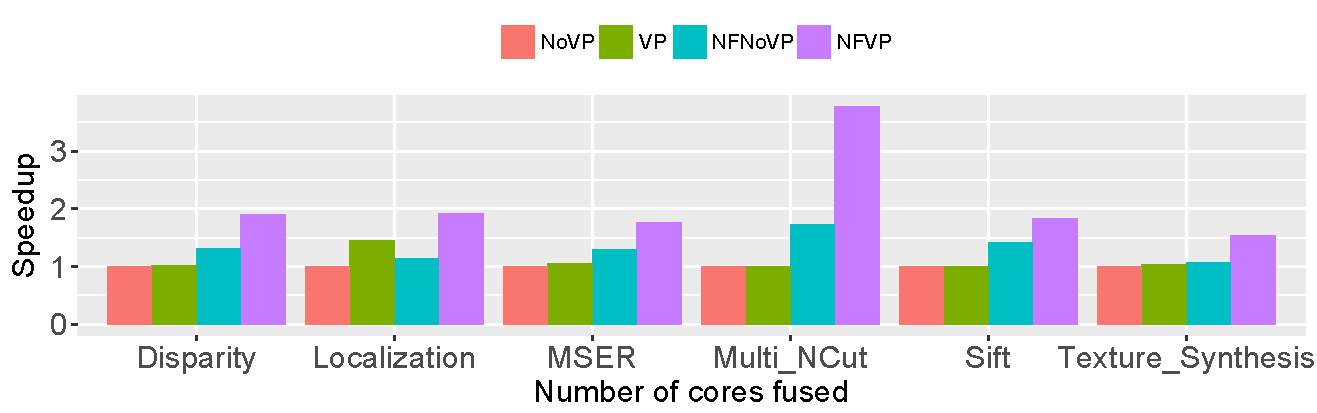
\includegraphics[width=1\textwidth]{chapter3/graphics/tempres.pdf}
    \caption{Comparing the performance of the standard fetching scheme to the new fetching scheme, with and without perfect value prediction. Higher is better}
    \label{fig:perf_pred}
	\vspace{1em}
\end{figure}

All configurations use perfect branch prediction.
Figure~\ref{fig:perf_pred} shows the speedup obtained on the SD-VBS benchmarks using the different configurations, with normal fetching scheme with no value prediction as a baseline.
The baseline is chosen as it represents a setup similar to the previous two chapters, the only difference being the perfrect branch prediction.
The number of cores composed for each benchmark using the different configurations can be found in Table~\ref{tab:conf_cores}.

\begin{table}[t]
  \small
  \centering
 \begin{tabular} {| l | l | l | l | l | l | }
 \hline
    & \cellcolor[gray]{0.7}Disparity & \cellcolor[gray]{0.7} Localization& \cellcolor[gray]{0.7} MSER& \cellcolor[gray]{0.7} Multi\_NCut& \cellcolor[gray]{0.7} Sift\\ \hline
 \textbf{\textit{NoVP}}   & 16  & 16 & 4  & 16& 16\\ \hline
 \textbf{\textit{VP}}   & 16  & 16 & 4  & 16& 16\\ \hline
 \textbf{\textit{NFNoVP}}   & 16  & 16 & 4  & 16& 16\\ \hline
 \textbf{\textit{NFVP}}   & 16  & 16 & 4  & 16& 16\\ \hline
	  & \cellcolor[gray]{0.7} Stitch & \cellcolor[gray]{0.7} SVM & \cellcolor[gray]{0.7} Text. Synth & \cellcolor[gray]{0.7} Tracking&\\ \hline
\textbf{\textit{NoVP}}	 & 16& 16& 16& 16 &\\ \hline
   \textbf{\textit{VP}} & 16  & 16 & 4  & 16 & \\ \hline
 \textbf{\textit{NFNoVP}}  & 16  & 16 & 4  & 16 & \\ \hline
 \textbf{\textit{NFVP}}   & 16  & 16 & 4  & 16 &\\ \hline

	\end{tabular}
  \caption{Number of cores composed for each SD-VBS benchmark given a configuration.}\label{tab:conf_cores}
  \vspace{2em}
\end{table}

As a first observation, it is clear that using the new fetching scheme with value prediction (\textit{\textbf{NFVP}}) always results in the best speedup compared to the baseline.
For \bm{Multi\_NCut}, performance is improved by almost 4x when using \textit{\textbf{NFVP}}.
This is a significant speedup, as Chapter~\ref{chp:cases} showed that \bm{Multi\_Ncut} was a difficult benchmark for core composition.
On average, \textit{\textbf{NFVP}} outperforms the baseline by a factor of 2x.

The results in Figure~\ref{fig:perf_pred} show that when the new fetching scheme is not paired with value prediction, the performance improvements are less important.
For example, \bm{Localization} only has a 1.10x speedup when using the \textbf{\textit{NFNoVP}} configuration, compared to the 1.90x of \textbf{\textit{NFVP}}.
This is due to the fact that whilst blocks do fetch faster, the register dependencies between blocks still limit the performance of core composition.
In fact, \textbf{\textit{VP}} outperforms \textbf{\textit{NFNoVP}}, which shows how improtant value prediction is for \bm{Localization}.

On the other hand, \bm{Multi\_NCut} with \textbf{\textit{NFNoVP}} has a 1.60x speedup compared to the baseline.
In this situation, this is because \bm{Multi\_NCut} has small blocks, on average less than 10 instructions long as seen in Chapter~\ref{chp:cases} Section~\ref{sec:expl}.
When blocks are uniformly small, value prediction will not help when using the normal fetching scheme, as the composition will never be full, thus explaining why \textbf{\textit{VP}} does not perform better than the baseline.

The performance of \textit{\textbf{VP}} compared to \textit{\textbf{NoVP}} can be surprising as the perfect value prediction does not appear to speed up execution.
Value prediction is most useful when multiple data-dependent blocks are in flight.
However, as seen in Section~\ref{chp3:sec:fetch} the normal fetching scheme is too slow to ensure that all cores in a composition are executing blocks.
Therefore, value prediction does not benefit baseline setup, as the large core compositions are never full.

\begin{figure}[t]
    \centering
    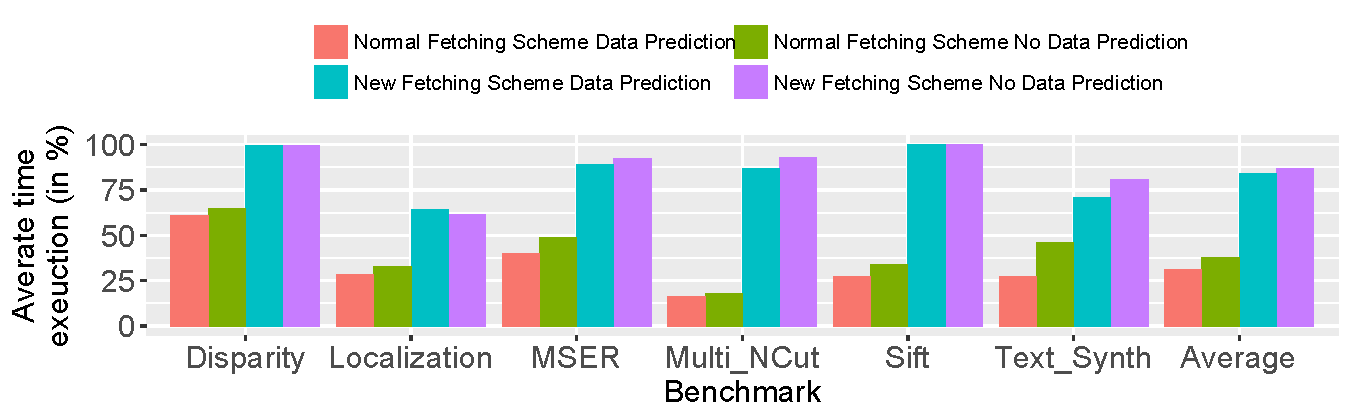
\includegraphics[width=1\textwidth]{chapter3/graphics/perf_av_cycle_exec.pdf}
    \caption{Average cycle yada}
    \label{fig:perf_av_cycle}
	\vspace{1em}
\end{figure}

To better highlight how the normal fetching scheme hinders performance even with value prediction the average \textit{active cycles} of each core in the composition, for each benchmark, is shown in Figure~\ref{fig:perf_av_cycle}.
For each configuration, the \textit{active cycles} of each core in the composition is averaged out and then compared to the total execution time of the application.
When the averaged \textit{active cycles} is close to the total execution time, this means that the composition was efficiently used, as each core executed the same amount of code.

As Figure~\ref{fig:perf_av_cycle} shows, \textbf{\textit{NoVP}} and \textbf{\textit{VP}} often have low active cycles compared to the total execution time.
This is due to the fact that block fetches are serialised, and thus, some cores will be innactive due to waiting for another core to send it a fetch request.
The lower the percentage is, the less likely there are going to be multiple blocks in flight which in turn means value prediction is less useful.


\subsection{Using perfect branch prediction and Block VTAGE value predictor}
\begin{figure}[t]
    \centering
    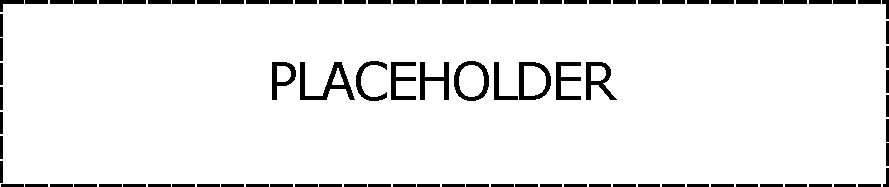
\includegraphics[width=1\textwidth]{chapter3/graphics/wip.pdf}
    \caption{Comparing the performance of the new fetching scheme, with perfect value prediction and with the VTAGE predictor. Higher is better}
    \label{fig:perf_pred}
	\vspace{1em}
\end{figure}

\subsection{Bottleneck analysis}